\documentclass{../slides}

\title{3827 OH}
\author{Eumin Hong (eh2890)}
\institute{Columbia University}
\date{February 15, 2022}

\begin{document}

\begin{frame}
    \titlepage
\end{frame}

\begin{frame}{Overview}
\begin{multicols}{2}
\tableofcontents
\end{multicols}
\end{frame}

\section{Announcements}
\subsection{Upcoming Assessments}
\begin{frame}{\secname: \subsecname}
    \begin{itemize}
        \item For HW2, do not hand in \enquote{Warmup Problems} -- answers are on CourseWorks
        \item HW3 is due on Friday 2/18
        \item HW4 is due on Friday 2/25
        \item Will have HW1 and HW2 graded soon
    \end{itemize}
\end{frame}

\subsection{Homework 1 and Homework Submission}
\begin{frame}{\secname: \subsecname}
    \begin{itemize}
        \item Common errors from Homework 1:
        \begin{itemize}
            \item Detecting when overflow happens (last two carries don't match)
            \item Missing bits in question 5 (floating point number) -- group bits in $4$
            \item Misinterpretation of signed magnitude/1's complement/2's complement
        \end{itemize}
        \item Submitting homework on Gradescope:
        \begin{itemize}
            \item Be sure you submit to the right TA and right homework number
            \item There are a lot of assignments, so just search for text
        \end{itemize}
    \end{itemize}
\end{frame}

\subsection{Feedback}
\begin{frame}{\secname: \subsecname}
    \begin{itemize}
        \item Form: \url{https://forms.gle/cnUmKVNYN7WvRbHA6}
        \item From feedback since last time:
        \begin{itemize}
            \item \enquote{...it would be nice if you asked for HW problems after 15 mins of going through the important concepts rather than spending 40+ mins on the important concepts and then remaining time on the hw.}
            \begin{itemize}
                \item Will start taking HW problems earlier and cover concepts as we go
                \item Will denote notable concepts with \enquote{NC}
            \end{itemize}
            \item \enquote{It also would be nice if when going through the concepts you do some example problems that are similar to the homework.}
            \begin{itemize}
                \item Coming up with questions is always hard, so I will probably default to using the homework questions to show concepts I am referring to
            \end{itemize}
        \end{itemize}
    \end{itemize}
\end{frame}

\section{Homework 3 Warmup}
\subsection{Problem 1}
\begin{frame}{\secname: \subsecname}
    Build a MUX from a Decoder and some AND and OR gates.
    \begin{itemize}
        \item NC: Symmetry of inputs and circuit logic
    \end{itemize}
\end{frame}

\subsection{Problem 2}
\begin{frame}{\secname: \subsecname}
    A MUX-with-Enable is a MUX with one additional selector input, $E$. When $E = 1$, the MUX-with-Enable behaves like a traditional MUX. When $E = 0$, the MUX-with-Enable is disabled and outputs $0$. Build a MUX-with-Enable from a MUX (without enable) and some AND gates.
\end{frame}

\subsection{Problem 3}
\begin{frame}{\secname: \subsecname}
    A $1$-to-$2^k$ DEMUX takes one data input $I$ and a $k$-bit selector $S$ as input and outputs $0$ on each of $2^k -1$ outputs, and outputs $I$ on the $j$th output where $j$ is the unsigned binary value represented by $S$. Construct a DEMUX from a decoder and a bunch of AND gates.
\end{frame}

\subsection{Problem 4}
\begin{frame}{\secname: \subsecname}
    Use five $2$-to-$1$ MUXs and as many NOT gates as needed, buid a circuit that take a $5$-bit value and a selector input $S$ and returns
    \begin{itemize}
        \item when $S = 0$, the original number is returned
        \item when $S = 1$, the $1$'s complement of the number is returned.
    \end{itemize}
    \begin{itemize}
        \item NC: MUXes as if/then/else statements
    \end{itemize}
\end{frame}

\subsection{Problem 5}
\begin{frame}{\secname: \subsecname}
    Build a circuit using two $2$-to-$1$ MUXs that takes a $2$ bit-input $B_1B_0$ and a $1$-bit selector $S$ and returns $B_1B_0$ when $S = 0$ and returns $B_0B_1$ (i.e., switches the bit-order) when $S = 1$.
    \begin{itemize}
        \item NC: MUXes as if/then/else statements
    \end{itemize}
\end{frame}

\subsection{Problem 6}
\begin{frame}{\secname: \subsecname}
    Solve problem 3 of the “Harder Problems” using four $16$-to-$1$ MUXs, one MUX for each output NSH, NSL, EWH, EWL. Now solve using four $8$-to-$1$ MUXs.
    \begin{itemize}
        \item NC: MUXes as brute-force solution
    \end{itemize}
\end{frame}

\subsection{Problem 7}
\begin{frame}{\secname: \subsecname}
    Design a circuit that receives a $k$-bit string $A = A_{k-1}A_{k-2}\dots A_1A_0$ and, using $k - 2$ $4$-to-$1$ MUXs, outputs $k$-bit string $B = B_{k-1}B_{k-2}\dots B_1B_0$ with the following properties
    \begin{itemize}
        \item $B_0 = A_0$, $B_{k-1} = A_{k-1}$
        \item $B_i = A_i$, whenever $A_{i+1}\neq A_{i-1}, 0 < i < k-1$
        \item $B_i = A_{i-1}$, whenever $A_{i+1} = A_{i-1}, 0 < i < k-1$
    \end{itemize}
    \begin{itemize}
        \item NC: MUXes as if/then/else statements
    \end{itemize}
\end{frame}

\section{Homework 3 Harder Problems}
\subsection{Problem 1}
\begin{frame}{\secname: \subsecname}
    Construct a $4$-to-$16$ line decoder with an enable input using five $2$-to-$4$ line decoders with enable inputs (Hint: Start at the outputs: If all that is being used is decoders, then how many decoders are connected directly to outputs?)
    \begin{itemize}
        \item NC: Symmetry of circuit
        \item NC: matching combinational circuits to number of inputs/outputs
        \item NC: partitioning of input (i.e. $I_3I_2I_1I_0$ into $I_3I_2$ and $I_1I_0$)
    \end{itemize}
\end{frame}

\subsection{Problem 2}
\begin{frame}{\secname: \subsecname}
    A combinatorial circuit is specified by the following three Boolean functions:
    \begin{gather*}
        F = X + \overbar{Y} + \overbar{X}YZ
    \end{gather*}
    Design the circuit with a decoder and external OR gates.
    \begin{itemize}
        \item NC: decoder as \enquote{cases} or minterms
    \end{itemize}
\end{frame}

\subsection{Problem 3}
\begin{frame}{\secname: \subsecname}
    A traffic light controller receives a $4$-bit input that changes every $5$ seconds. The input sequence is a simple counter that counts from binary $0$ to binary $15$ and then starts again from binary $0$. These signals go to $4$ outputs, NSH, NSL, EWH, EWL. The first two outputs NSH and NSL respectively represent the high and low bits that are fed to the lamps that face in the North-south direction. The other two outputs EWH and EWL respectively represent the high and low bits that are fed to the lamps that face in the East-West direction. The following table indicates how setting the high and low bits determines the color of the lamp:
    \begin{figure}[H]
        \centering
        \begin{tabular}{cc|c}
            High & Low & Lamp Color \\ \hline 
            $0$ & $1$ & Yellow \\
            $1$ & $0$ & Red \\
            $1$ & $1$ & Red
        \end{tabular}
    \end{figure}
\end{frame}

\begin{frame}{\secname: \subsecname\ (cont.)}
    Each light should be green for $30$ seconds, yellow for $5$ seconds, and then red for $45$ seconds. There should be two $5$ second intervals when both lights are red. Assume that for the interval where the input is $0000$, the North-South light has just turned green, and the East-West light has been red for $5$ seconds already.

    Design the circuitry that feeds from $ABCD$ to the two outputs. You may represent your answer as algebraic equations (make sure to simplify).
    \begin{itemize}
        \item NC: at least one similar word problem (probably with FSMs) will be on exam
    \end{itemize}
\end{frame}

\subsection{Problem 4}
\begin{frame}{\secname: \subsecname}
    The $01$-swap operation, $b$, on a binary string $S$, permutes all occurences of $01$ within the original string to $10$ (the process is not recursive). For instance:
    \begin{itemize}
        \item $b(0) = 0, b(1) = 1, b(00) = 00, b(01) = 10, b(11) = 11$
        \item $b(000) = 000, b(001) = 010, b(010) = 100, b(100) = 100$
        \item $b(0\ 01\ 01\ 1\ 01\ 0) = 0\ 10\ 10\ 1\ 10\ 0$ (spacing added for clarity)
    \end{itemize}
    Design a circuit using $2$:$1$ multiplexers that can be used to perform the $01$-swap on a $k$-bit string $S = S_{k-1}S_{k-2}\dots S_0$. where each $S_i$ is a bit.
\end{frame}

\begin{frame}{\secname: \subsecname\ (cont.)}
    \begin{enumerate}[(a)]
        \item First, show the circuit, built using the $2$:$1$ MUX, whose output is the $i$th bit of $b(S)$ where $0 < i < k - 1$. YOU DO NOT NEED ANY AND, OR, OR NOT GATES, only a single $2$:$1$ MUX. This is somewhat challenging, so think what input information you need.
        \item Use contraction to solve the edge cases when $i = 0, k - 1$. You do not have to simplify the internals of the MUX, just explain why you \enquote{contracted} as you did.
    \end{enumerate}
    \begin{itemize}
        \item NC: solving parts of larger question will appear on exam
        \item NC: contraction is setting certain inputs to constants and/or getting rid of unnecessary components
    \end{itemize}
\end{frame}

\subsection{Problem 5}
\begin{frame}{\secname: \subsecname}
    The isolated-$1$-shift-left operationg (i$1$sl for short) applied to a binary string $S$ moves a $1$ bit by one position to the left in the solution if the bit is not adjacent to any other $1$'s (i.e., $0$'s on both sides, or if is the least-significant bit, a $0$ immediately above it).

    For instance, the following show application of i$1$sl to various strings:
    \begin{itemize}
        \item $010\to 100, 011\to 011, 01010\to 10100$
        \item $011010\to 011100, 011100\to 011100$
    \end{itemize}
    \begin{enumerate}[(a)]
        \item Build a simplified circuit (using only AND, OR, NOT gates) whose output is the $i$th bit of the i$1$sl, where $1 < i < k-1$ (there's a hint here about what inputs are needed). You may leave your answer in algebraic (SoP) form in terms of the $S_j$. Note that the $i$th bit can be determined by only looking at a few of the $S_j$.
    \end{enumerate}
\end{frame}

\begin{frame}{\secname: \subsecname\ (cont.)}
    \begin{enumerate}[(a)]
    \setcounter{enumi}{1}
        \item Suppose it is known that the input string will never contain $3$ consecutive $1$'s. Draw the simplified circuit.
        \item Suppose the input string might contain $3$ $1$'s, but that no consecutive $4$ bits contain $3$ $0$'s (i.e., $0000$, $0001$, $0010$, $0100$, or $1000$ never appear as a substring), nor does $0101$ ever appear ($1010$ might still apear though, e.g., $111011011010$). Draw the simplified circuit.
        \item Use contraction to design the circuits for the outputs of the $k-1$th, $1$st, $0$th bits.
    \end{enumerate}
    \begin{itemize}
        \item NC: contraction is setting certain inputs to constants and/or getting rid of unnecessary components
    \end{itemize}
\end{frame}

\section{Homework 4 Topics}
\subsection{SR Latch}
\begin{frame}{\secname: \subsecname}
    \begin{itemize}
        \item Latches just hold state -- can be changed by changing the values of the inputs
        \item SR latch has inputs of \enquote{Set} ($S$) and \enquote{Reset} ($R$)
        \item SR latch has outputs of $Q$ and $\overbar{Q}$
    \end{itemize}
    \begin{figure}[H]
        \centering
        \begin{tikzpicture}[circuit logic US, label distance=2mm]
            \node (r) at (0, 3) {$R$};
            \node (s) at (0, 0) {$S$};
            \node[nor gate, draw] (n1) at (2, 2.5) {};
            \node[nor gate, draw] (n2) at (2, 0.5) {};
            \node (q) at (4.5, 2.5) {$Q$};
            \node (q') at (4.5, 0.5) {$\overbar{Q}$};
            \draw (n1.output) -- (q) ;
            \draw (n2.output) -- (q') ;
            \draw (r) --(1, 3) |- (n1.input 1);
            \draw (s) --(1, 0) |- (n2.input 2);
            \draw (3.5, 2.5) -- (3.5, 2.25) -- (1, 1) |- (n2.input 1);
            \draw (3.5, 0.5) -- (3.5, 0.75) -- (1, 2) |- (n1.input 2);
            \draw[black,fill=black] (3.5, 2.5) circle (0.05) node[anchor=south east] {};
            \draw[black,fill=black] (3.5, 0.5) circle (0.05) node[anchor=south east] {};
        \end{tikzpicture}
    \end{figure}
    \begin{itemize}
        \item For understanding behavior of circuit for given $(R, S)$, think about when NOR operation gives $0$
        \begin{itemize}
            \item Or more generally, passing a constant to a gate can make its output constant as well
        \end{itemize}
    \end{itemize}
\end{frame}

\subsection{D Latch}
\begin{frame}{\secname: \subsecname}
    \begin{itemize}
        \item Basically SR latch with some more circuitry to avoid \enquote{illegal} combinations of inputs (e.g. when $R = 1, S = 1$ what does the SR latch do? How can it \enquote{set} $Q = 1$ and \enquote{reset} $Q = 0$ at the same time?)
        \item D latch has inputs $D$ and $C$ (control, which ensures $S\neq R$ in the underlying SR latch)
        \begin{itemize}
            \item $D$ is the value to store/write if $C = 1$
            \item $C$ can also be $E$ for enable
        \end{itemize}
    \end{itemize}
\end{frame}

\subsection{Clocking}
\begin{frame}{\secname: \subsecname}
    \begin{multicols}{2}
        \begin{itemize}
            \item Clock signal oscillates between $0$ and $1$ with a fixed period
            \begin{itemize}
                \item \enquote{Rising edge} of clock signal is the transition from \enquote{low} to \enquote{high} (i.e. $0\to 1$)
            \end{itemize}
            \begin{figure}[H]
                \centering
                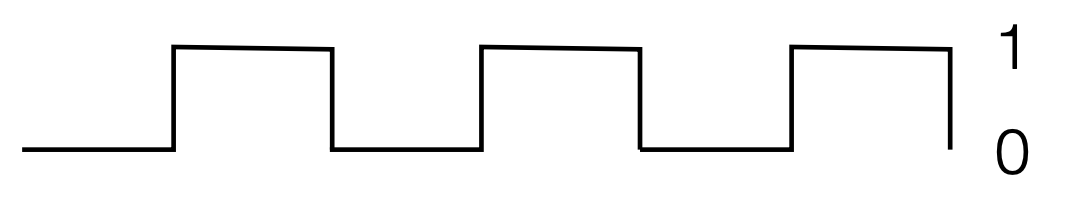
\includegraphics[width = 4cm]{img/clock.png}
            \end{figure}
            \begin{itemize}
                \item Kind of like a metronome, gives the circuit a sense of time on which it can operate
            \end{itemize}
            \begin{itemize}
                \item Why should I care about clock? It determines the rate at which instructions are executed
            \end{itemize}
            \begin{figure}[H]
                \centering
                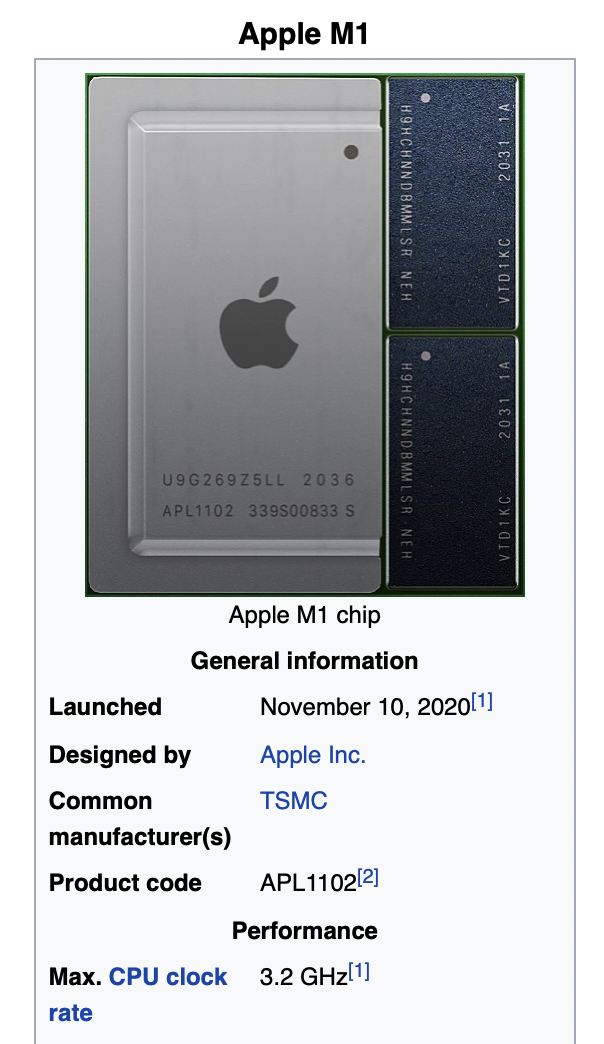
\includegraphics[width = 4cm]{img/m1.png}
            \end{figure}
        \end{itemize}
    \end{multicols}
\end{frame}


\subsection{Flip-Flops}
\begin{frame}{\secname: \subsecname}
    \begin{itemize}
        \item Latches do not support clocking individually
        \item Connecting latches in series (and ensuring that the clock inputs are complemented or staggered) acts as a flip-flop
        \item Example of D Flip-Flop:
        \begin{figure}[H]
            \centering
            \tikzset{flipflop DC/.style={flipflop, flipflop def={t1=D, t2=C, t6=Q, t4={\ctikztextnot{Q}}}}}
            \begin{tikzpicture}[circuit logic US, label distance=2mm]
                \node[flipflop DC] (D1) at (0, 0) {};
                \node[flipflop DC] (D2) at (4, 0) {};
                \node (s) at (-3, 0.84) {$S$};
                \node (c) at (-3, 0) {$CLK$};
                \node (q) at (6, 0.84) {$Q$};
                \node (q') at (6, -0.84) {$\overbar{Q}$};
                \node[not gate, draw] (not) at (0, -2) {};
                \draw (s) -- (D1.pin 1);
                \draw (c) -- (D1.pin 2);
                \draw (D1.pin 6) -- (D2.pin 1);
                \draw (D2.pin 6) -- (q);
                \draw (D2.pin 4) -- (q');
                \draw (-2, 0) |- (not.input);
                \draw (not.output) -| (2, 0) -- (D2.pin 2);
                \draw[black,fill=black] (-2, 0) circle (0.05) node[anchor=south east] {};
            \end{tikzpicture}
        \end{figure}
        \item Left D latch is updated when $CLK = 1$ (new inputs read to left D latch), right D latch is updated when $CLK = 0$ (load new inputs to right D latch)
    \end{itemize}
\end{frame}

\subsection{Flip-Flop Behavior}
\begin{frame}{\secname: \subsecname}
    \begin{itemize}
        \item For the D flip-flop:
        \begin{figure}[H]
            \centering
            \begin{tabular}{c|c}
                $D(t)$ & $Q(t + 1)$\\\hline
                $0$ & $0$ \\
                $1$ & $1$
            \end{tabular}
        \end{figure}
        \item The input $t$ is time, or more specifically, the $t$th clock cycle
        \begin{itemize}
            \item A clock cycle is one period of the clock
        \end{itemize}
        \item In other words, the input $D$ at clock cycle $t$ becomes the output $Q$ at clock cycle $t+1$ (the next clock cycle)
    \end{itemize}
\end{frame}

\subsection{Flip-Flop Abstraction}
\begin{frame}{\secname: \subsecname}
    \begin{itemize}
        \item The two latch circuit from earlier is abstracted and is a D flip-flop (D since it has the same inputs as a D latch) (left circuit)
        \begin{figure}[H]
            \centering
            \begin{tikzpicture}[circuit logic US, label distance=2mm]
                \node[flipflop D] () at (0, 0) {};
                \node[flipflop D, add async SR] () at (4, 0) {};
            \end{tikzpicture}
        \end{figure}
        \item The triangular input (bottom left) is for the clock signal
        \item How do we initialize the values of a flip-flop?
        \begin{itemize}
            \item Use set and reset inputs (right circuit), implementation is not necessary to know (we are not really worried about initialization in this course)
        \end{itemize}
    \end{itemize}
\end{frame}

\end{document}
